\begin{refsection}
\chapter{Introduction to \texttt{IsoplotR}}
\label{ch:intro2IsoplotR}
  
For many years, a \texttt{Microsoft Excel} add-in called
\texttt{Isoplot} has been the main data processing software of choice
in geochronology. Developed by Kenneth R. Ludwig over a period of two
decades, \texttt{Isoplot} is a user-friendly toolbox that allows
geologists to calculate and visualise geochronological data within a
familiar spreadsheet environment \citep{ludwig1988, ludwig1999,
  ludwig2003, ludwig2012}.  Few computer programs have been as widely
used in the Earth Sciences as \texttt{Isoplot}. Written in Visual
Basic for Applications (\texttt{VBA}), \texttt{Isoplot} takes isotopic
data as input and produces publication-ready figures as output.\\

Unfortunately, recent versions of \texttt{Excel} are incompatible with
\texttt{Isoplot}, whose creator has retired and no longer maintains
the code. These software issues are a major problem for the field of
radiometric geochronology, to the point where some laboratories kept
an old \texttt{Windows~XP} computer with \texttt{Excel~2003} around
for the sole purpose of running \texttt{Isoplot}.\\

\texttt{IsoplotR} is a free, open and more future proof alternative
for \texttt{Isoplot} \citep{vermeesch2018c}.  \texttt{IsoplotR}'s
software architecture uses a modular design with future proofness and
extendability in mind.

\section{Software architecture}
\label{sec:architecture}

There are three ways to use \texttt{IsoplotR}: online, offline and
from the command line.\\

The online
version\footnote{\texttt{http://isoplotr.london-geochron.com/}} is
convenient in several ways. First, it requires no software
installation. Second, the \texttt{IsoplotR} website is perfectly
platform-independent. It renders on any modern HTML-5 compatible web
browser, including those installed on smartphones and tablet
computers. Third, by using the online version, the user is guaranteed
to have accessed the most up-to-date version of the software.\\

An offline version of the GUI is provided for use on computers that
are not (permanently) connected to the internet. This is often the
case for machines that are connected to mass spectrometers, as a
safety precaution. The offline version of the GUI works by emulating a
web server within the default browser on the user's
system. Installation instructions are provided on the
\texttt{IsoplotR} website and on
\texttt{GitHub}\footnote{\texttt{https://github.com/pvermees/IsoplotRgui/}}.\\

The third way to access the full functionality of \texttt{IsoplotR} is
through the command line within the \texttt{R} programming
environment. The command line offers the greatest flexibility to
automate, modify and extend \texttt{IsoplotR}'s functionality.

\section{The Graphical User Interface (GUI)}
\label{sec:GUI}

The code base for the GUI and the core data processing algorithms are
surgically separated. The command-line functionality is grouped in a
lightweight package called \texttt{IsoplotR} that may be installed
from CRAN as instructed in
Section~\ref{sec:R}.\ref{it:installingIsoplotR}. The \texttt{IsoplotR}
package has minimal dependencies and should work on a basic \texttt{R}
installation. In contrast, the GUI is written in \texttt{HTML} and
\texttt{Javascript} and interacts with \texttt{IsoplotR} via an
interface package. It is provided in a second \texttt{R} package
called \texttt{IsoplotRgui} that is available from CRAN as well:

\begin{console}
> install.packages('IsoplotRgui')
\end{console}

Once installed, \texttt{IsoplotRgui} can be started from the
\texttt{R} console as follows:

\begin{console}
> library(IsoplotRgui)
> IsoplotR()
\end{console}

This opens the GUI in a new tab of the user's default internet
browser.  The GUI has four components: a top bar with selection menus
for the various chronometers and plot devices, optional settings and
documentation; an input table into which data can be pasted from
spreadsheet applications; an output window displaying the graphical or
numerical results; and a lower bar to import and export data and
results:\\

\noindent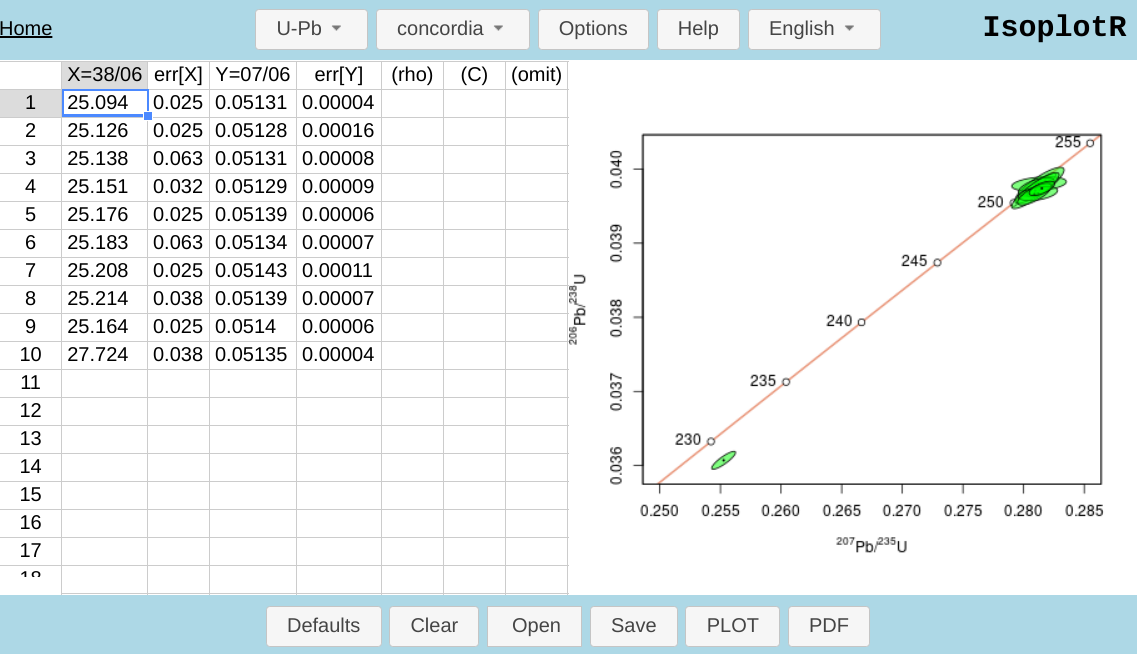
\includegraphics[width=\textwidth]{../figures/IsoplotR.png}\\

\noindent\begin{minipage}[t]{.15\textwidth}
\strut\vspace*{-\baselineskip}\newline
  
\includegraphics[width=.7\linewidth]{../figures/chronometerbutton.png}
\end{minipage}
\begin{minipage}[t]{.85\textwidth}
IsoplotR currently implements 12 different geochronometers: U--Pb,
Pb--Pb, Th--Pb, Ar--Ar, K--Ca, Rb--Sr, Sm--Nd, Re--Os, Lu--Hf,
U--Th--He, fission tracks, and Th--U.  Additionally, it also includes
functionality for detrital geochronology and general purpose data
processing.\\
\end{minipage}

\noindent\begin{minipage}[t]{.15\textwidth}
\strut\vspace*{-\baselineskip}\newline

\includegraphics[width=\textwidth]{../figures/plotdevices.png}
\end{minipage}
\begin{minipage}[t]{.85\textwidth}
For each chronometer there are several possible plot devices.  These
may vary from method to method. For example, concordia plots are only
available for U--Pb data, and release spectra for Ar--Ar data.\\
\end{minipage}

\noindent\begin{minipage}[t]{.15\textwidth}
\strut\vspace*{-\baselineskip}\newline

\includegraphics[width=.7\textwidth]{../figures/Options.png}
\end{minipage}
\begin{minipage}[t]{.85\textwidth}
The \texttt{Options} menu allows the user to choose between different
input formats and change parameters (e.g. decay constants, plot
colours) that affect the numerical or graphical output.\\
\end{minipage}

\noindent\begin{minipage}[t]{.15\textwidth}
\strut\vspace*{-\baselineskip}\newline

\includegraphics[width=.55\textwidth]{../figures/Help.png}
\end{minipage}
\begin{minipage}[t]{.85\textwidth}
The \texttt{Help} button provides further information about the input
table, about the graphical and numerical numerical results, and some
references. The \texttt{Help} function dynamically responds to the
settings that are listed under the \texttt{Options} menu.\\
\end{minipage}

\noindent\begin{minipage}[t]{.15\textwidth}
\strut\vspace*{-\baselineskip}\newline

\includegraphics[width=.55\textwidth]{../figures/Open.png}\\

\includegraphics[width=.55\textwidth]{../figures/Save.png}\\
\end{minipage}
\begin{minipage}[t]{.85\textwidth}
The data and settings can be stored in a \texttt{.json} format for
further processing in the future.\\
\end{minipage}

\noindent\begin{minipage}[t]{.15\textwidth}
\strut\vspace*{-\baselineskip}\newline

\includegraphics[width=.55\textwidth]{../figures/PLOT.png}\\

\includegraphics[width=.55\textwidth]{../figures/RUN.png}\\
\end{minipage}
\begin{minipage}[t]{.85\textwidth}
The \texttt{PLOT} button (or \texttt{RUN} button if \texttt{ages} or
`\texttt{get $\zeta$}' is chosen as output) saves all the current
settings and produces the graphical and/or numerical output.\\
\end{minipage}

\noindent\begin{minipage}[t]{.15\textwidth}
\strut\vspace*{-\baselineskip}\newline

\includegraphics[width=.55\textwidth]{../figures/PDF.png}\\

\includegraphics[width=.55\textwidth]{../figures/CSV.png}\\
\end{minipage}
\begin{minipage}[t]{.85\textwidth}
Clicking the \texttt{PDF} button repeats the calculations but saves
the output as a \texttt{.pdf} file, which can be further processed by
vector editing software such as \texttt{Adobe Illustrator},
\texttt{CorelDraw} or \texttt{Inkscape}. If \texttt{ages} is chosen as
output saves the results to a comma separated value (\texttt{.csv})
file.\\
\end{minipage}

\noindent\begin{minipage}[t]{.15\textwidth}
\strut\vspace*{-\baselineskip}\newline
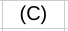
\includegraphics[width=.55\textwidth]{../figures/C.png}\\
\end{minipage}
\begin{minipage}[t]{.85\textwidth}
The \texttt{(C)} column of the input table can be used to store
numerical values that can be used as a fill colour for the plot
symbols.\\
\end{minipage}

\noindent\begin{minipage}[t]{.15\textwidth}
\strut\vspace*{-\baselineskip}\newline
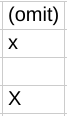
\includegraphics[width=.55\textwidth]{../figures/omit.png}
\end{minipage}
\begin{minipage}[t]{.85\textwidth}
Specific samples can be omitted from the numerical calculations
(e.g. isochron, weighted mean, or concordia age) by marking them with
a lowercase `x' in the optional \texttt{(omit)} column. To hide
samples from the graphical (as well as the numerical) output, mark
them with an uppercase `X'.\\
\end{minipage}

\noindent\begin{minipage}[t]{.25\textwidth}
\strut\vspace*{-\baselineskip}\newline
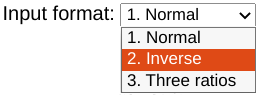
\includegraphics[width=\textwidth]{../figures/formats.png}
\end{minipage}
\begin{minipage}[t]{.75\textwidth}
The \texttt{Options} menu provides access to a range of different
input formats. Selecting any item from this menu replaces the input
table with a different set of default data.\\
\end{minipage}

\noindent\begin{minipage}[t]{.25\textwidth}
\strut\vspace*{-\baselineskip}\newline
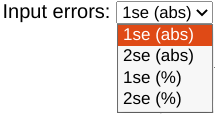
\includegraphics[width=.85\textwidth]{../figures/ierr.png}
\end{minipage}
\begin{minipage}[t]{.75\textwidth}
The \texttt{Options} menu also allows the user to specify the ratio
uncertainties as being absolute or relative errors at 1 or 2 standard
errors. Selecting any item from this menu automatically changes the
input data accordingly.\\
\end{minipage}

\noindent\begin{minipage}[t]{.25\textwidth}
\strut\vspace*{-\baselineskip}\newline
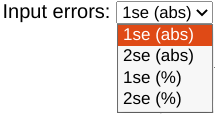
\includegraphics[width=.85\textwidth]{../figures/ierr.png}\\
\end{minipage}
\begin{minipage}[t]{.75\textwidth}
Contextual help can be obtained by clicking any text string within the
\texttt{Options} menu.
\end{minipage}

\noindent\begin{minipage}[t]{.45\textwidth}
\strut\vspace*{-\baselineskip}\newline
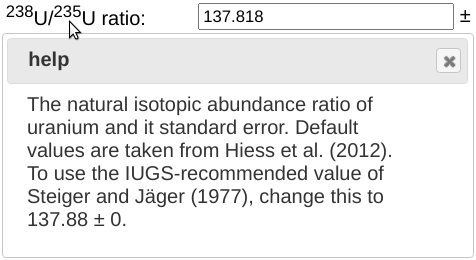
\includegraphics[width=\textwidth]{../figures/contextualhelp.png}
\end{minipage}
\begin{minipage}[t]{.55\textwidth}
Contextual help can be obtained by clicking any text string within the
\texttt{Options} menu.
\end{minipage}

\section{The Command Line Interface (CLI)}

CLI offers all the functionality of the GUI, and more. A complete list
of public functions can be viewed by typing

\begin{console}
> help(package='IsoplotR')
\end{console}

\noindent at the command prompt. Data are read from comma-separated
variable (\texttt{.csv}) files using the \texttt{read.data()}
function. For example:

\begin{script}
UPb_dat <- read.data('file.csv',method='U-Pb',format=1,ierr=3)
\end{script}

\noindent where\\

\noindent\begin{tabular}{@{}p{.2\textwidth}@{}p{.04\textwidth}@{}p{.76\textwidth}@{}}
\verb|'file.csv'| && is the name of the data
file\\ \verb|method='U-Pb'| && specifies the
chronometer\\ \verb|format=1| && tells \texttt{IsoplotR} that
\verb|file.csv| contains the following columns:
\textsuperscript{207}Pb/\textsuperscript{235}U,
err[\textsuperscript{207}Pb/\textsuperscript{235}U],
\textsuperscript{206}Pb/\textsuperscript{238}U,
err[\textsuperscript{206}Pb/\textsuperscript{238}U], and $r$, where
`err[*]' marks the uncertainties of `*', and $r$ is the correlation
coefficient between
err[\textsuperscript{207}Pb/\textsuperscript{235}U] and
err[\textsuperscript{206}Pb/\textsuperscript{238}U] (see
Chapter~\ref{ch:statistics}).\\ \verb|ierr=3| && indicates that these
uncertainties (`err[*]') are specified as relative values at two
standard errors.
\end{tabular}\\

\noindent Further details about these arguments can be viewed by
typing \texttt{?read.data} at the console. The various plot devices
are implemented in a collection of designated functions such as
\texttt{concordia()}, \texttt{isochron()}, \texttt{weightedmean()},
\texttt{isochron()}, \texttt{agespectrum()}, \texttt{KDE()},
\texttt{CAD()} and \texttt{radialplot()} that will be discussed in
further details in later chapters. A table of age estimates can be
obtained using the \texttt{ages()} function. Many of
\texttt{IsoplotR}'s functions are \emph{overloaded}, which means that
the same function can be applied to multiple data types with
potentially different results. For example, using the output of
\verb|read.data('data.csv',method='Rb-Sr')| as input to the
\texttt{isochron()} function automatically produces a Rb--Sr isochron,
with the correct decay constants and axis labels.\\

A colour scale can be added to most plots using the options
\texttt{levels} argument. For example:

\begin{script}[firstnumber=2]
ns <- length(UPb_dat)
concordia(UPb_dat,levels=runif(ns),ellipse.fill=c("yellow","red")
\end{script}

\noindent assigns a vector of random numbers to some U--Pb data and
uses these numbers to colour the error ellipses on a concordia diagram
from yellow to red. Omitting or hiding samples from calculations
and/or plots is achieved by specifying the indices of the relevant
aliquots to the functions of interest. For example:

\begin{script}[firstnumber=2]
weightedmean(UPb_dat,omit=10)
\end{script}

\noindent omits the 10\textsuperscript{th} from the weighted mean
calculation, whereas

\begin{script}[firstnumber=2]
weightedmean(UPb_dat,hide=10)
\end{script}

\noindent removes the aliquot from the weighted mean diagram
altogether.\\

The GUI may be the easiest way to interact with \texttt{IsoplotR} and
explore various data processing strategies with individual
samples. But the CLI is more useful than the GUI when processing large
datasets comprising multiple samples, and provides a powerful
mechanism to produce \emph{reproducible} science. The \texttt{.csv}
data files and \texttt{.R} data processing scripts can easily be
archived and shared with others. They provide a parsimonious way to
produce FAIR science \citep{wilkinson2016}.

\printbibliography[heading=subbibliography]
\end{refsection}
